\documentclass[UKenglish]{article}  %% ... or USenglish or norsk
\usepackage[utf8]{inputenc}
\usepackage[T1]{url}

\usepackage[a4paper]{geometry}
\usepackage{listings}

\setlength{\parskip}{1em}
\setlength{\parindent}{0em}
\usepackage{caption}
\usepackage{subcaption}

\urlstyle{sf}
\usepackage{babel}
\usepackage{graphicx}
\usepackage{ifikompendiumforside}
\usepackage{hyperref}
\usepackage{tikz}
\usepackage{array}
\usepackage[font={small,it,sf}]{caption}
\usepackage{longtable}
\usepackage{wrapfig}
\usetikzlibrary{arrows, shadows}

\title{INF4121 Project Assignment 1}
\subtitle{Interpret the metrics offered by the static analyzer}
\author{Per Øyvind Karlsen, Melat Fisseha Tekelmichael}

\begin{document}
\ififorside

\section{Introducion}

\subsection{Objective}
The objective of the assignment is to discover what the source code does and
test it manually. This source code then needs to be analyzed using a static
analyzer tool called “Source Monitor”. The tool will help us obtain some
code metrics and interpret them based on the project under analysis to see its
weak parts of the code. The weak points then need to be improved and measure
it again to see the improved metrics.
The main aim will then be to compare the two interpretations of these metrics. 

\subsection{Project selection}
The Java implementation of Minesweeper was the project we chose to analyze for
our assignment and is available on github:

\url{https://github.com/proyvind/inf3121}

\section{Requirement 1}

\subsection{Brief description}
The project we chose consists of three files: “MineField.java”,
“Ranking.java” and a test program  “Minesweeper.java”.
Each file is constructed with having only one class.
The project is a game called Minesweeper where a player is initially presented
with a grid of undifferentiated squares. Some randomly selected squares,
unknown to the player, are designated to contain mines.
Typically, the size of the grid and the number of mines are set in advance by
the user, either by entering the numbers or selecting from defined skill
levels, depending on the implementation. The number of mines, is equivalent to
1/3 the number of squares, or less.

\url{https://en.wikipedia.org/wiki/Minesweeper_(video_game)}

\subsection{Analysis of testable parts}
In order to test its functionality we have used black-box testing. Here we test
the input and see the output we get. We chose the \textbf{Boundary value analysis}
and \textbf{Equivalence class partitioning} techniques.
We have also used two factors that will help us analyse the testable parts.
\textbf{Observability}: where this shows us the degree of possibility to observe the
test results.
\textbf{Understandability}: to check if the component is self-explaining. 
\textbf{Usability}: 

As non- functional testing tests the quality characteristics of the component,
it would not make sense not to write a non-functional tests. 
Though it covers the aspects of the product that may not relate to a specific
function, it still tests the aspects like reliability, usability, portability
and many more. As to the program that i have selected to this assignment, I
would say to write a non-functional test. To ground the argument let us assume
that a customer needs to include this game in his/ her casino house.
The owner that’s going to buy the product needs to know  if the these type
of tests has been performed.

\subsection{Non-functional tests}

\subsubsection{Performance, load and stress}

\subsubsection{Reliability}

\subsubsection{Usability}

\subsubsection{Efficiency}

\subsubsection{Maintainability}

\subsubsection{Portability}

\subsection{Test cases}

\section{Requirement 2}

\subsection{Metrics at project level}
For our use of SourceManager for this project, a few details should be
mentioned to explain the metrics initially measured.
For the SourceMonitor project options, we used modified complexity metric
(count switch/case as only one statement), didn't count blank lines for lines
metric and also ignored header \& footer comment.
The reasoning for this is to ensure complexity metric better reflects
readabiliy of code, while also avoid that lines of code that usually helps
making code easier to read doesn't affect lines metric.
Besides these personal choices affecting the metrics, there was also a bug
in SourceMonitor triggered by the initialization of arrays in the MineField()
constructor that broke the metrics reported for this file. In order to work
around this bug the relevant code was moved into a separate function called by
the constructor.

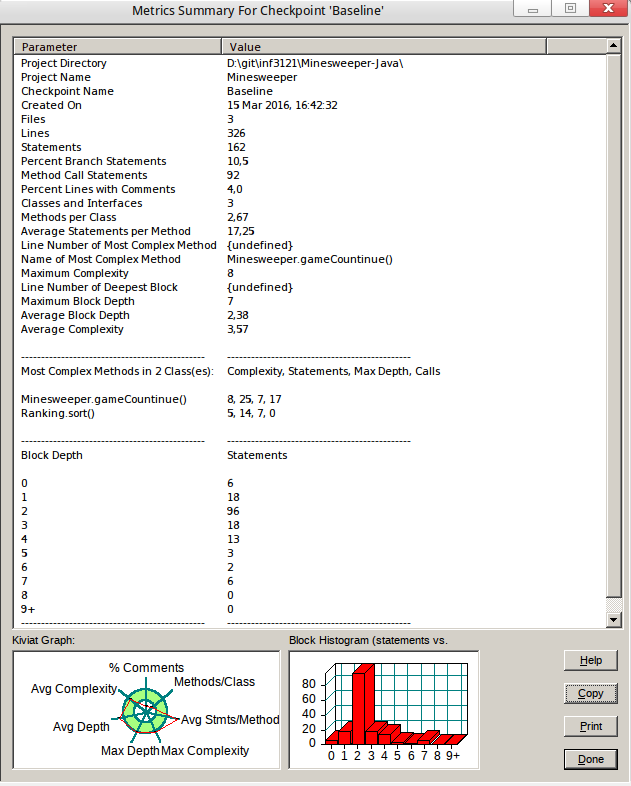
\includegraphics[height=12cm]{project-metrics-summary-original.png}

The application of metrics interpretations can vary when applied in class, file
or method. For this project, we will use list of metrics. And we here by list
out some of the metrics with their interpretation;

\begin{longtable}[H]{| m{1in} |  m{2in} | m{2in} |}
	\hline
	\textbf{Metric} & \textbf{Description} & \textbf{Explanation}\\
	\hline Percent Lines with Comments & Tells how much of the code that
	are made up of comments. & For this project comments makes up 4.8\% of
	all it's code.\\
	\hline Methods per Class & The number of methods in each class of a
	file. In cases of more than one class it is the average of methods in
	all the classes. & In this case it is 5.33.\\
	\hline Average Statements per Method & The total number of statements
	in all methods divided by the number of methods. & For this project this
	is 10.38.\\
	\hline Maximum complexity & Complexity is simply the number of decision
	structures in a method. Maximum complexity is/are the most complex
	method(s) of a file/class. & In this project it is found to be 12.\\
	\hline Maximum Block Depth & The depth measures the number of blocks
	in a method. The maximum block depth then tells us the deepest methods
	of a class. & For this project it is 7.\\
	\hline Average Block Depth & The total of all enclosed blocks depth amount
	divided by depth. & For this project it is 2.73.\\
	\hline Average Complexity & Calculated by dividing the total of each
	method’s complexity by the number of methods. & For this project it is
	3.38.\\
	\hline
\end{longtable}

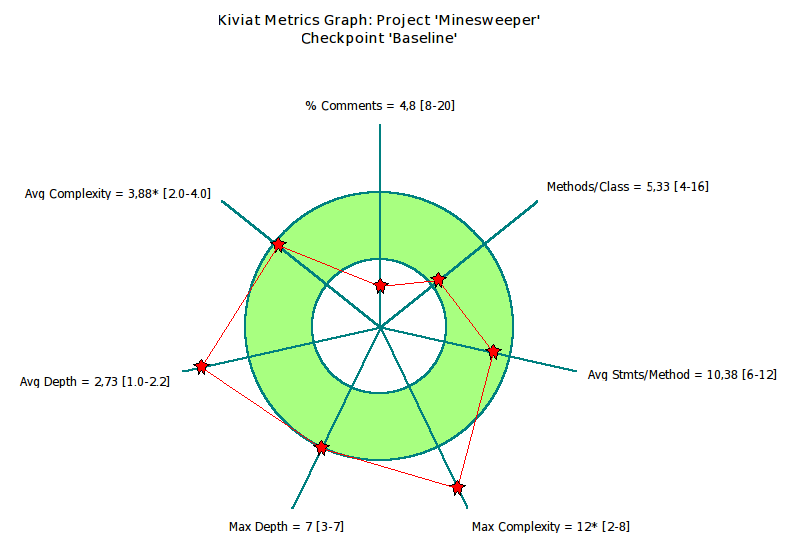
\includegraphics[height=8cm]{project-kiviat-metrics-graph-original.png}
The measurement is shown in a kiviat graph. A kiviat graph is a tool that
visually displays a set of metrics that provides easy viewing of multiple
metrics against minimum and maximum thresholds.  All metrics are scaled so
that all maximums are in a common circle and the same for minimums.
The metrics are the radials in the circle. The big circle is the maximum
threshold and the small circle is the minimum. The metrics values that are
with these two circles are the acceptable values that doesn’t need
improvement. If not, it needs improvement.

\subsubsection{Biggest file by the number of lines of code}
The biggest file we have in the project is “MineField.java”. It contains 134 lines of code.

\subsubsection{File with most branches}
“MineField.java” has most percentage of branches in this project. It consists of 34.9\% branches.

\subsubsection{File with most complex code}
"MineField.java" is the file with complex code. It's average complexity of 4.11 is the metric we concluded this from.

\subsection{Metrics at file level}

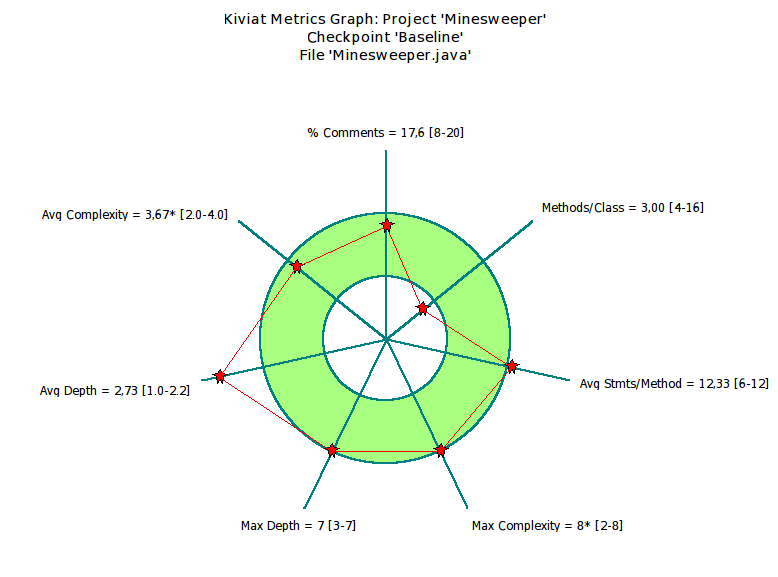
\includegraphics[height=8cm]{Minesweeper_java-kiviat-metrics-graph-original.png}

\end{document}
